% =============================================================================
% CAPÍTULO 2 - BLOQUE 2.5: SISTEMAS RAG MULTIMODALES (mRAG), COMPRENSIÓN DE
% VÍDEO LARGO, ANCLAJE ESPACIOTEMPORAL Y CUELLOS DE BOTELLA PERCEPTIVOS
% =============================================================================

\subsection{Sistemas RAG Multimodales (mRAG) y Comprensión de Vídeo de Larga Duración}
\label{subsec:sistemas_mrag}

\subsubsection{Arquitecturas de Referencia en Comprensión de Vídeo: \textit{Video-RAG}, \textit{CARVE} y \textit{Multi-RAG}}
\label{subsubsec:arquitecturas_videorag_carve_multirag}

La evolución de los sistemas de Recuperación Aumentada por Generación (RAG) ha transitado desde arquitecturas puramente textuales hacia paradigmas multimodales capaces de procesar, alinear e interpretar información visual, auditiva y textual dentro de un único espacio semántico continuo \cite{prajwal2025multimodal, multi_rag2025}. %[cite: 3, 5]
En el dominio específico de la recuperación de eventos sobre secuencias de vídeo de larga duración (\textit{Long-form Video Understanding}), esta transición permite localizar sucesos puntuales mediante consultas en lenguaje natural sin depender de metadatos anotados manualmente antes de la indexación \cite{video_rag2024}. %[cite: 3, 6]

Dentro de la literatura científica consolidada entre 2024 y 2026, destacan tres marcos arquitectónicos que abordan de manera complementaria la alineación visual, la granularidad temporal y la robustez operativa \cite{video_rag2024, multi_rag2025}: %[cite: 3, 5]

\begin{itemize}
    \item \textbf{Marco \textit{Video-RAG} (\textit{Visually-aligned Retrieval-Augmented Long Video Comprehension}):} Propone una arquitectura de recuperación alineada visualmente que complementa los fotogramas del vídeo mediante la extracción e indexación paralela de tres canales auxiliares: texto visible en pantalla obtenido por OCR, transcripciones auditivas y metadatos estructurados de detección de objetos \cite{video_rag2024}. %[cite: 3]
    Al recuperar conjuntamente las señales visuales y sus descriptores alineados, el sistema reduce la carga de contexto sobre el modelo generativo al analizar vídeos extensos \cite{video_rag2024}. %[cite: 3]
    \item \textbf{Sistema \textit{CARVE} (\textit{Cross-Modal and Multi-Granularity Retrieval}):} Aborda el problema de que los eventos de interés en un vídeo no poseen una duración uniforme —algunos sucesos duran apenas un segundo (como un gesto o la aparición fugaz de una línea de código) mientras que otros abarcan varios minutos (como la explicación completa de un diagrama)—. %[cite: 3, 6]
    \textit{CARVE} introduce un mecanismo de recuperación intermodal multigranular capaz de evaluar simultáneamente distintas escalas temporales, logrando superar de forma consistente a los métodos tradicionales de ventana única en métricas estándar de ordenación como \textbf{\textit{Recall@5}} y \textbf{\textit{nDCG@5}}. %[cite: 3]
    \item \textbf{Plataforma \textit{Multi-RAG} (\textit{Adaptive Video Understanding}):} Introduce una capa de aplicación práctica concebida como soporte cognitivo para la interacción humano-robot sobre flujos de vídeo capturados en tiempo real en entornos dinámicos y no estructurados \cite{multi_rag2025, arxiv_adaptive_2505}. %[cite: 5]
    Su principal aportación científica reside en demostrar que las representaciones vectoriales multimodales mantienen una inferencia semántica de alto rendimiento incluso cuando la señal visual se encuentra temporalmente degradada o limitada, evidenciando la viabilidad de los \textit{embeddings} multimodales bajo fuertes restricciones de recursos \cite{multi_rag2025}. %[cite: 5]
\end{itemize}

La Figura~\ref{fig:arquitecturas_videorag_carve_multirag} sintetiza los principios de diseño de estos tres sistemas de referencia en el estado del arte. %[cite: 3, 5]

\begin{figure}[htbp]
\centering
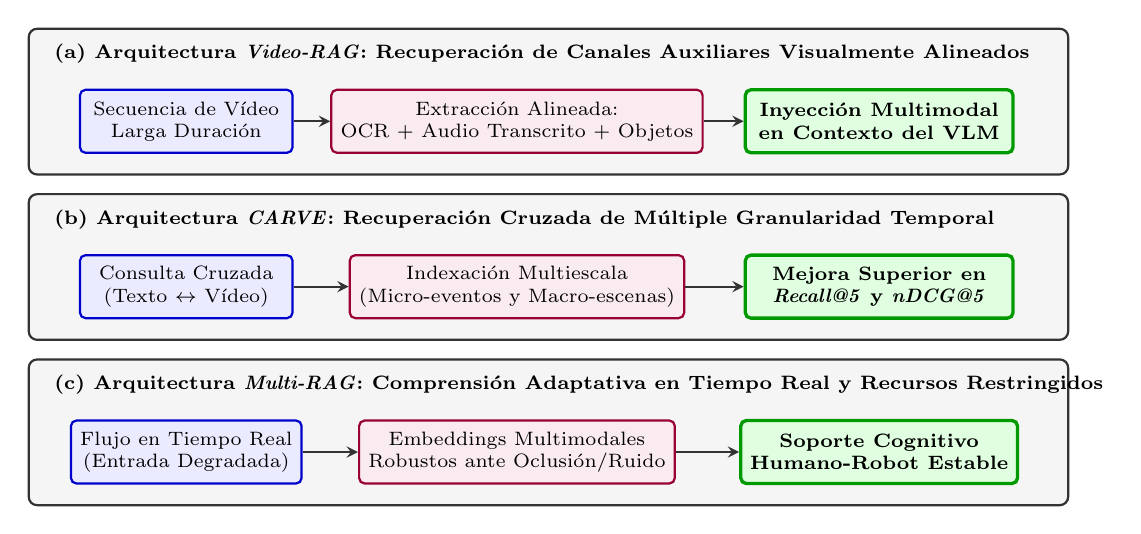
\begin{tikzpicture}[
    node distance=0.45cm and 0.6cm,
    archbox/.style={rectangle, draw=black!80, fill=gray!8, thick, minimum width=13.2cm, minimum height=1.85cm, rounded corners=3pt},
    innode/.style={rectangle, draw=blue!80!black, fill=blue!8, thick, minimum width=2.7cm, minimum height=0.8cm, align=center, font=\scriptsize, rounded corners=2pt},
    midnode/.style={rectangle, draw=purple!80!black, fill=purple!8, thick, minimum width=3.6cm, minimum height=0.8cm, align=center, font=\scriptsize, rounded corners=2pt},
    outnode/.style={rectangle, draw=green!60!black, fill=green!12, very thick, minimum width=3.4cm, minimum height=0.8cm, align=center, font=\scriptsize\bfseries, rounded corners=2pt},
    arrow/.style={-stealth, thick, draw=black!80}
]
% Video-RAG
\node[archbox] (b1) at (0, 4.2) {};
\node[font=\scriptsize\bfseries, anchor=north west] at (-6.4, 5.05) {(a) Arquitectura \textit{Video-RAG}: Recuperación de Canales Auxiliares Visualmente Alineados};
\node[innode] (v1_in) at (-4.6, 3.95) {Secuencia de Vídeo\\Larga Duración};
\node[midnode] (v1_mid) at (-0.4, 3.95) {Extracción Alineada:\\OCR + Audio Transcrito + Objetos};
\node[outnode] (v1_out) at (4.2, 3.95) {Inyección Multimodal\\en Contexto del VLM};
\draw[arrow] (v1_in) -- (v1_mid);
\draw[arrow] (v1_mid) -- (v1_out);

% CARVE
\node[archbox] (b2) at (0, 2.1) {};
\node[font=\scriptsize\bfseries, anchor=north west] at (-6.4, 2.95) {(b) Arquitectura \textit{CARVE}: Recuperación Cruzada de Múltiple Granularidad Temporal};
\node[innode] (v2_in) at (-4.6, 1.85) {Consulta Cruzada\\(Texto $\leftrightarrow$ Vídeo)};
\node[midnode] (v2_mid) at (-0.4, 1.85) {Indexación Multiescala\\(Micro-eventos y Macro-escenas)};
\node[outnode] (v2_out) at (4.2, 1.85) {Mejora Superior en\\\textit{Recall@5} y \textit{nDCG@5}};
\draw[arrow] (v2_in) -- (v2_mid);
\draw[arrow] (v2_mid) -- (v2_out);

% Multi-RAG
\node[archbox] (b3) at (0, 0.0) {};
\node[font=\scriptsize\bfseries, anchor=north west] at (-6.4, 0.85) {(c) Arquitectura \textit{Multi-RAG}: Comprensión Adaptativa en Tiempo Real y Recursos Restringidos};
\node[innode] (v3_in) at (-4.6, -0.25) {Flujo en Tiempo Real\\(Entrada Degradada)};
\node[midnode] (v3_mid) at (-0.4, -0.25) {Embeddings Multimodales\\Robustos ante Oclusión/Ruido};
\node[outnode] (v3_out) at (4.2, -0.25) {Soporte Cognitivo\\Humano-Robot Estable};
\draw[arrow] (v3_in) -- (v3_mid);
\draw[arrow] (v3_mid) -- (v3_out);
\end{tikzpicture}
\caption{Comparativa de tres arquitecturas representativas de sistemas RAG de vídeo en la literatura reciente: (a) alineación de metadatos auxiliares en \textit{Video-RAG}, (b) indexación multigranular en \textit{CARVE} y (c) inferencia adaptativa resiliente en \textit{Multi-RAG} \cite{video_rag2024, multi_rag2025}.} %[cite: 3, 5]
\label{fig:arquitecturas_videorag_carve_multirag}
\end{figure}

\subsubsection{Del Emparejamiento Semántico al Anclaje Causal Espaciotemporal (\textit{Temporal Grounding})}
\label{subsubsec:anclaje_causal_espaciotemporal}

El avance conceptual más profundo que caracteriza a la generación actual de sistemas Video RAG es el desplazamiento cualitativo desde el ``análisis temático'' hacia el verdadero \textbf{razonamiento y anclaje causal espaciotemporal (\textit{Temporal Grounding})} \cite{mixpeek_chunking, gemini_emb2_docs}. %[cite: 5, 6]
Los sistemas RAG tradicionales aplicados a multimedia se limitaban a responder preguntas resumiendo la temática general de un archivo (por ejemplo, devolver una síntesis genérica indicando que \textit{``el vídeo debate sobre economía''}). %[cite: 5]

Por el contrario, la convergencia de la fragmentación semántica adaptativa (\textit{Video-RAC}), los modelos de transcripción con alineación forzada (\textit{WhisperX}) y la diarización acústica de hablantes con modelos de \textit{embeddings} omnimodales permite que las arquitecturas contemporáneas formulen aserciones fundamentadas con precisión de milisegundos sobre la línea de tiempo \cite{video_rac2025, mixpeek_chunking}: %[cite: 5]

\begin{quote}
\textit{``Exactamente en el segmento 14:32, el segundo hablante señala el cuadrante superior derecho de la tabla, y el gráfico de barras indica un descenso de los ingresos, lo cual contradice el resumen textual proporcionado al inicio de la sesión''} \cite{mixpeek_chunking}. %[cite: 5]
\end{quote}

En este paradigma de \textit{grounding} temporal, el modelo cognitivo no inventa relaciones abstractas ni realiza aproximaciones difusas: se posiciona sobre un eje cronológico determinista $[t_{\text{inicio}}, t_{\text{fin}}]$ y discrimina el orden causal de los acontecimientos dentro de secuencias densas \cite{gemini_emb2_docs, mixpeek_chunking}. %[cite: 5, 6]
La Figura~\ref{fig:emparejamiento_vs_grounding_temporal} contrasta la salida de un sistema de emparejamiento temático clásico frente a un motor dotado de anclaje causal espaciotemporal. %[cite: 5, 6]

\begin{figure}[htbp]
\centering
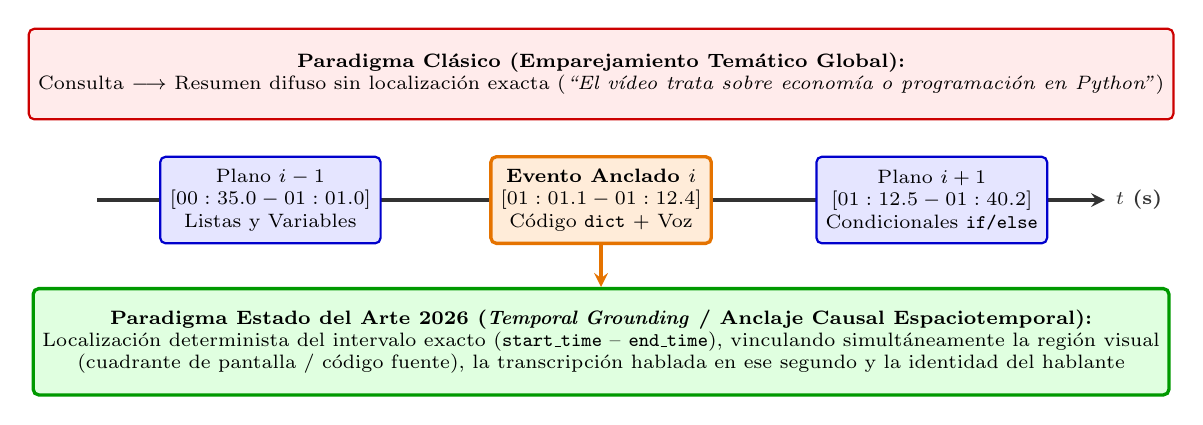
\begin{tikzpicture}[
    node distance=0.5cm and 0.7cm,
    oldbox/.style={rectangle, draw=red!80!black, fill=red!8, thick, minimum width=12.8cm, minimum height=1.15cm, align=center, font=\scriptsize, rounded corners=2pt},
    timebox/.style={rectangle, draw=blue!80!black, fill=blue!10, thick, minimum width=2.8cm, minimum height=1.1cm, align=center, font=\scriptsize, rounded corners=2pt},
    groundbox/.style={rectangle, draw=green!60!black, fill=green!12, very thick, minimum width=12.8cm, minimum height=1.35cm, align=center, font=\scriptsize, rounded corners=2pt},
    arrow/.style={-stealth, thick, draw=black!80}
]
% Paradigma Antiguo
\node[oldbox] (old) at (0, 2.3) {\textbf{Paradigma Clásico (Emparejamiento Temático Global):}\\
Consulta $\longrightarrow$ Resumen difuso sin localización exacta (\textit{``El vídeo trata sobre economía o programación en Python''})};

% Línea de tiempo determinista
\draw[-stealth, very thick, black!80] (-6.4, 0.7) -- (6.4, 0.7) node[right, font=\scriptsize\bfseries] {$t$ (s)};
\node[timebox] (c1) at (-4.2, 0.7) {Plano $i-1$\\$[00:35.0 - 01:01.0]$\\Listas y Variables};
\node[timebox, draw=orange!90!black, fill=orange!15, very thick] (c2) at (0.0, 0.7) {\textbf{Evento Anclado $i$}\\$[01:01.1 - 01:12.4]$\\Código \texttt{dict} + Voz};
\node[timebox] (c3) at (4.2, 0.7) {Plano $i+1$\\$[01:12.5 - 01:40.2]$\\Condicionales \texttt{if/else}};

% Paradigma Grounding Temporal
\node[groundbox] (new) at (0, -1.1) {\textbf{Paradigma Estado del Arte 2026 (\textit{Temporal Grounding} / Anclaje Causal Espaciotemporal):}\\
Localización determinista del intervalo exacto (\texttt{start\_time} -- \texttt{end\_time}), vinculando simultáneamente la región visual\\(cuadrante de pantalla / código fuente), la transcripción hablada en ese segundo y la identidad del hablante};

\draw[arrow, very thick, orange!90!black] (c2.south) -- (new.north);
\end{tikzpicture}
\caption{Contraste entre el emparejamiento temático tradicional y el Anclaje Causal Espaciotemporal (\textit{Temporal Grounding}), el cual proporciona trazabilidad determinista y auditable sobre la línea de tiempo del vídeo \cite{mixpeek_chunking, gemini_emb2_docs}.} %[cite: 5, 6]
\label{fig:emparejamiento_vs_grounding_temporal}
\end{figure}

Esta capacidad de anclaje milimétrico y judicialmente auditable habilita cinco dominios estratégicos de aplicación documentados en el proyecto \cite{gemini_emb2_docs}: %[cite: 5, 6]
\begin{enumerate}
    \item \textbf{Educación y Repositorios Académicos (RAG de Clases Grabadas):} Permite a un estudiante consultar \textit{``minuto donde el profesor explica la mitosis usando el diagrama en la pizarra''} o localizar el instante exacto en que un tutorial de programación explica cómo construir listas, diccionarios o condicionales \texttt{if/else}, razonando sobre la conjunción del audio y el código en pantalla. %[cite: 3, 6]
    \item \textbf{Auditoría de Seguridad y Videovigilancia:} Capacidad para inspeccionar cientos de horas de cámaras de seguridad sin supervisión humana mediante consultas en lenguaje natural como \textit{``coche rojo saltándose un semáforo a gran velocidad''} o \textit{``persona abandonando una mochila gris''}, recuperando las marcas de tiempo exactas. %[cite: 6]
    \item \textbf{Gestión de Archivos de Medios y \textit{Broadcasting}:} Localización instantánea en archivos históricos de televisión mediante búsquedas que combinan carga visual y entonación acústica, tales como \textit{``momentos de tensión en debates políticos''} o \textit{``personas llorando de alegría''}. %[cite: 6]
    \item \textbf{Análisis de Historiales Médicos y Diagnóstico Continuo:} Construcción de un perfil vectorial unificado que proyecta los informes clínicos en texto libre junto con las pruebas diagnósticas de imagen (radiografías, resonancias o ecografías) para encontrar casos clínicos equivalentes o auditar secuencias médicas. %[cite: 5, 6]
    \item \textbf{Comercio Electrónico y Búsqueda Visual Cruzada:} Recuperación de artículos específicos en catálogos multimedia a partir de una fotografía o una nota de voz descriptiva del usuario (\textit{``busco un sofá verde esmeralda de terciopelo con patas de madera''}). %[cite: 6]
\end{enumerate}

\subsubsection{Cuellos de Botella Perceptivos en la Verificación Visual: Resolución Espacial y Compresión JPEG}
\label{subsubsec:cuellos_botella_perceptivos_ocr}

Si bien la teoría de los modelos fundacionales multimodales postula la eliminación de los motores OCR tradicionales gracias a la lectura directa de parches visuales \cite{prajwal2025multimodal}, la experimentación empírica en sistemas reales revela que el \textbf{OCR implícito} de un modelo de visión-lenguaje es altamente sensible a las transformaciones de preprocesamiento de imagen aplicadas en el \textit{pipeline} de ingestión. %[cite: 3, 5]

En una arquitectura de búsqueda en dos etapas que utiliza \textit{Gemini Embedding 2} (vía Qdrant) para recuperar los fragmentos candidatos y emplea un modelo ligero secundario (\textit{Gemini 1.5 Flash Lite} o \textit{Gemini Flash 3.5}) como verificador visual para descartar falsos positivos, un ajuste agresivo de los hiperparámetros de codificación visual induce fallos críticos de falso rechazo (falsos negativos). %[cite: 3]

Durante las pruebas empíricas sobre el vídeo de validación \texttt{python\_tutorial.mp4} (\textit{``Python en 8 Minutos''}), al ejecutar la consulta \texttt{"Diccionarios"}, el motor vectorial recuperó en la quinta posición el intervalo temporal $01\text{:}01.1\text{ -- }01\text{:}40.2$ ($61,1\text{ s -- }100,2\text{ s}$). %[cite: 3]
Aunque la verdad terreno (\textit{ground truth}) del vídeo muestra explícitamente en pantalla entre los segundos $01\text{:}01.0$ y $01\text{:}03.0$ la sintaxis de un diccionario en Python (\texttt{dict \{"name": "Brais"\}}), el verificador visual descartó erróneamente el fragmento emitiendo el diagnóstico: \textit{``Descartado (Falso Positivo: 0\%) -- Análisis visual: El segmento cubre listas y variables, pero no muestra diccionarios''}. %[cite: 3]

La auditoría técnica de los parámetros de indexación demuestra que este fallo perceptivo responde a dos cuellos de botella en la codificación de los fotogramas clave antes de su envío a la API: %[cite: 3]
\begin{enumerate}
    \item \textbf{Resolución espacial destructiva (\texttt{resize\_width = 512}\text{ px}):} Redimensionar un videotutorial grabado en alta definición —donde el código fuente ocupa una fracción reducida del editor en pantalla— a un ancho máximo de $512$ píxeles reduce la altura de las tipografías a apenas unos pocos píxeles borrosos. %[cite: 3]
    Incluso manteniendo una calidad JPEG alta ($80$), a $512\text{ px}$ los caracteres de la palabra reservada \texttt{dict} y las llaves \texttt{\{\}} pierden su definición geométrica, impidiendo que tanto \textit{Gemini Embedding 2} como \textit{Gemini Flash} puedan leer la sintaxis. %[cite: 3]
    \item \textbf{Cuantización JPEG agresiva (\texttt{jpeg\_quality = 12} o \texttt{20}):} Cuando además de baja resolución se aplica un factor de calidad JPEG extremo ($12$ o $20$ en la escala $1\text{--}100$ de \texttt{cv2.imencode}), los macrobloques de la Transformada Discreta del Coseno (DCT) difuminan por completo los bordes de alto contraste del texto sobre el fondo del editor, convirtiendo el código en un artefacto ilegible. %[cite: 3]
\end{enumerate}

La Figura~\ref{fig:cuello_botella_ocr_implicito} esquematiza el mecanismo exacto por el cual la degradación de resolución y compresión induce alucinaciones de descarte en el verificador visual, así como los rangos de calibración óptimos. %[cite: 3]

\begin{figure}[htbp]
\centering
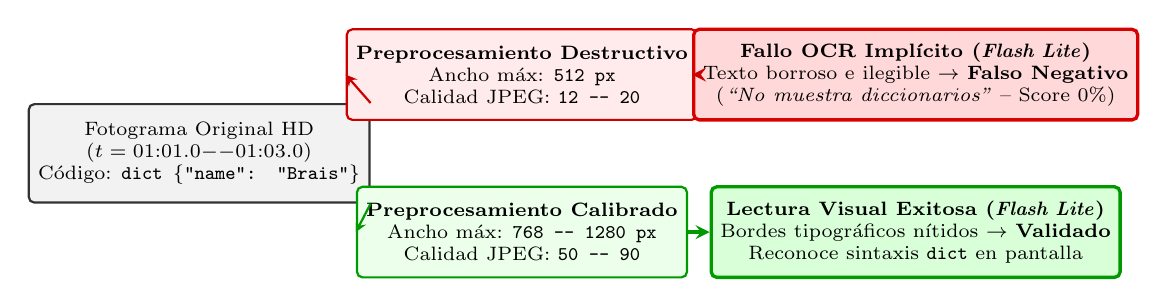
\begin{tikzpicture}[
    node distance=0.5cm and 0.65cm,
    srcbox/.style={rectangle, draw=black!80, fill=gray!10, thick, minimum width=2.8cm, minimum height=1.25cm, align=center, font=\scriptsize, rounded corners=2pt},
    badproc/.style={rectangle, draw=red!80!black, fill=red!8, thick, minimum width=3.4cm, minimum height=1.15cm, align=center, font=\scriptsize, rounded corners=2pt},
    goodproc/.style={rectangle, draw=green!60!black, fill=green!8, thick, minimum width=3.4cm, minimum height=1.15cm, align=center, font=\scriptsize, rounded corners=2pt},
    badout/.style={rectangle, draw=red!85!black, fill=red!15, very thick, minimum width=4.5cm, minimum height=1.15cm, align=center, font=\scriptsize, rounded corners=2pt},
    goodout/.style={rectangle, draw=green!60!black, fill=green!15, very thick, minimum width=4.5cm, minimum height=1.15cm, align=center, font=\scriptsize, rounded corners=2pt},
    arrow/.style={-stealth, thick, draw=black!80}
]
\node[srcbox] (frame) at (-5.2, 0.0) {Fotograma Original HD\\($t = 01\text{:}01.0\text{ -- }01\text{:}03.0$)\\Código: \texttt{dict \{"name": "Brais"\}}};

% Rama Superior: Degradación Crítica
\node[badproc] (b_enc) at (-1.1, 1.0) {\textbf{Preprocesamiento Destructivo}\\Ancho máx: \texttt{512 px}\\Calidad JPEG: \texttt{12 -- 20}};
\node[badout] (b_vlm) at (3.9, 1.0) {\textbf{Fallo OCR Implícito (\textit{Flash Lite})}\\Texto borroso e ilegible $\to$ \textbf{Falso Negativo}\\(\textit{``No muestra diccionarios''} -- Score 0\%)};

% Rama Inferior: Calibración Óptima
\node[goodproc] (g_enc) at (-1.1, -1.0) {\textbf{Preprocesamiento Calibrado}\\Ancho máx: \texttt{768 -- 1280 px}\\Calidad JPEG: \texttt{50 -- 90}};
\node[goodout] (g_vlm) at (3.9, -1.0) {\textbf{Lectura Visual Exitosa (\textit{Flash Lite})}\\Bordes tipográficos nítidos $\to$ \textbf{Validado}\\Reconoce sintaxis \texttt{dict} en pantalla};

\draw[arrow, red!80!black, thick] (frame.north east) -- (b_enc.west);
\draw[arrow, red!80!black, very thick] (b_enc.east) -- (b_vlm.west);
\draw[arrow, green!60!black, thick] (frame.south east) -- (g_enc.west);
\draw[arrow, green!60!black, very thick] (g_enc.east) -- (g_vlm.west);
\end{tikzpicture}
\caption{Diagnóstico del cuello de botella perceptivo en la etapa de verificación visual: el escalado a $512\text{ px}$ combinado con compresión JPEG agresiva ($12\text{--}20$) impide el OCR implícito de sintaxis de programación en pantalla, mientras que elevar \texttt{resize\_width} al rango $768\text{--}1280\text{ px}$ y la calidad JPEG a $50\text{--}90$ restaura la detección sin disparar el consumo de cuota.} %[cite: 3]
\label{fig:cuello_botella_ocr_implicito}
\end{figure}

\subsubsection{Dilución Semántica en Fragmentos de Larga Duración y Muestreo Estático de Fotogramas}
\label{subsubsec:dilucion_semantica_muestreo}

El segundo fenómeno crítico identificado durante la validación del sistema es el problema de la \textbf{dilución semántica y pérdida de fotogramas clave} en fragmentos de larga duración. %[cite: 3]
En vídeos con un fondo visual altamente estático —tales como clases grabadas, presentaciones de diapositivas o tutoriales de código donde el entorno gráfico del editor permanece inalterado y únicamente cambian unas pocas líneas de texto—, el índice de similitud estructural (SSIM) entre fotogramas consecutivos se mantiene elevado durante largos periodos. %[cite: 3]

Cuando el umbral de corte SSIM se configura en un valor demasiado permisivo (\texttt{threshold = 0.08}) o incluso en un valor moderado (\texttt{threshold = 0.60}) sin imponer una duración máxima de plano, el algoritmo agrupa secuencias extensas en un único \texttt{VideoChunk} —como el citado fragmento \#5 de $39,1$ segundos de duración ($01\text{:}01.1\text{ -- }01\text{:}40.2$)—. %[cite: 3]
A una cadencia estándar de $f_{\text{fps}} = 30$ fotogramas por segundo, un fragmento de $\Delta T = 39,1\text{ s}$ contiene un total de $N_{\text{total}} = \Delta T \times f_{\text{fps}} \approx 1.173$ fotogramas. %[cite: 3]
Dado que la función \texttt{extract\_key\_frames} selecciona un número estático de $k = 3$ fotogramas por fragmento (inicial, final y máxima entropía), la fracción de cobertura temporal cae drásticamente, provocando dos efectos adversos: %[cite: 3]
\begin{itemize}
    \item \textbf{Omisión por submuestreo (\textit{Keyframe Miss}):} Si el evento buscado (la escritura de \texttt{dict \{"name": "Brais"\}}) ocurre entre los segundos $01\text{:}01.0$ y $01\text{:}03.0$, pero el fotograma de máxima entropía global de esos $39,1$ segundos recae en el segundo $01\text{:}25.0$ (donde la pantalla está más llena de código de listas o variables), ninguno de los $3$ fotogramas enviados a la API contendrá el diccionario. %[cite: 3]
    \item \textbf{Dilución del vector agregado en el espacio latente:} Al mezclar en un único \texttt{VideoChunk} casi $40$ segundos que abarcan múltiples subtemas distintos (variables, listas y diccionarios), el vector resultante en \textit{Gemini Embedding 2} promedia todas esas temáticas, perdiendo especificidad direccional frente a consultas puntuales. %[cite: 3]
\end{itemize}

La Figura~\ref{fig:dilucion_semantica_chunks_largos} ilustra gráficamente cómo se produce esta pérdida por muestreo en un \textit{chunk} gigante y cómo la corrigen las estrategias de acotación temporal o muestreo dinámico. %[cite: 3]

\begin{figure}[htbp]
\centering
\begin{tikzpicture}[scale=0.95]
% Caso A: Chunk Gigante (39.1s) con pérdida de fotograma clave
\node[font=\scriptsize\bfseries, anchor=west] at (0, 2.5) {(a) Fragmento Masivo sin Límite Superior ($\Delta T = 39,1\text{ s}$, Umbral SSIM $= 0,08 / 0,60$ en vídeo estático):};
\draw[fill=red!8, draw=red!80!black, thick, rounded corners=2pt] (0, 1.3) rectangle (12.6, 2.2);
\node[font=\scriptsize, red!80!black] at (6.3, 1.75) {\texttt{VideoChunk \#5} ($01\text{:}01.1 \longrightarrow 01\text{:}40.2$) --- Mezcla Variables, Listas y Diccionarios (Dilución Semántica)};

% Zona donde ocurre realmente el diccionario
\draw[fill=yellow!35, draw=orange!90!black, very thick] (0.2, 1.3) rectangle (1.3, 2.2);
\node[above, font=\tiny\bfseries, orange!90!black] at (0.75, 2.2) {Evento \texttt{dict} ($01\text{:}03$)};

% Los 3 fotogramas muestreados (F1, F_entropia, F3) que fallan el evento
\filldraw[blue!80!black] (0.05, 1.75) circle (3pt) node[below=4pt, font=\tiny\bfseries] {$F_{\text{ini}}$};
\filldraw[blue!80!black] (7.8, 1.75) circle (3pt) node[below=4pt, font=\tiny\bfseries] {$F_{\text{entropía}}$ (Listas)};
\filldraw[blue!80!black] (12.55, 1.75) circle (3pt) node[below=4pt, font=\tiny\bfseries] {$F_{\text{fin}}$};

% Caso B: Corrección mediante max_shot_frames (10-15s) o Muestreo Proporcional
\node[font=\scriptsize\bfseries, anchor=west] at (0, 0.35) {(b) Solución Arquitectónica: Corte Forzado por Duración Máxima (\texttt{max\_shot\_frames} $\approx 10\text{--}15\text{ s}$) o Muestreo Dinámico:};
\draw[fill=green!12, draw=green!60!black, very thick, rounded corners=2pt] (0, -0.8) rectangle (3.1, 0.05);
\node[font=\tiny\bfseries, green!50!black] at (1.55, -0.37) {Sub-Chunk 5a ($01\text{:}01\text{--}01\text{:}11$): \textbf{Captura \texttt{dict}}};

\draw[fill=gray!12, draw=black!70, thick, rounded corners=2pt] (3.2, -0.8) rectangle (6.3, 0.05);
\node[font=\tiny] at (4.75, -0.37) {Sub-Chunk 5b ($01\text{:}11\text{--}01\text{:}21$)};

\draw[fill=gray!12, draw=black!70, thick, rounded corners=2pt] (6.4, -0.8) rectangle (9.5, 0.05);
\node[font=\tiny] at (7.95, -0.37) {Sub-Chunk 5c ($01\text{:}21\text{--}01\text{:}31$)};

\draw[fill=gray!12, draw=black!70, thick, rounded corners=2pt] (9.6, -0.8) rectangle (12.6, 0.05);
\node[font=\tiny] at (11.1, -0.37) {Sub-Chunk 5d ($01\text{:}31\text{--}01\text{:}40$)};
\end{tikzpicture}
\caption{Mecanismo de dilución semántica y pérdida de fotogramas clave en vídeos con baja variación visual: (a) un fragmento de casi $40\text{ s}$ muestreado con solo $3$ fotogramas omite el instante en que aparece el diccionario y mezcla múltiples temas; (b) la imposición de un límite superior (\texttt{max\_shot\_frames} de $10\text{--}15\text{ s}$) o la extracción proporcional (un fotograma extra cada $5\text{ s}$) garantiza la cohesión semántica.} %[cite: 3]
\label{fig:dilucion_semantica_chunks_largos}
\end{figure}

El Cuadro~\ref{tab:diagnostico_parametros_visuales} resume la comparativa técnica entre las configuraciones defectuosas analizadas durante la depuración y los rangos corregidos necesarios para preservar tanto la legibilidad del texto en pantalla como la granularidad temporal de los fragmentos. %[cite: 3]

\begin{table}[htbp]
\centering
\caption{Diagnóstico empírico de parámetros de preprocesamiento visual y temporal en sistemas Video RAG con verificación secundaria (\textit{Gemini Embedding 2} + \textit{Gemini Flash}) \cite{gemini_emb2_docs}.} %[cite: 3]
\label{tab:diagnostico_parametros_visuales}
\begin{tabular}{llll}
\hline
\textbf{Parámetro del Pipeline} & \textbf{Config. Defectuosa} & \textbf{Efecto Patológico en el RAG} & \textbf{Configuración Óptima Calibrada} \\
\hline
Ancho máx. (\texttt{resize\_width}) & $512\text{ px}$ & Texto/código ilegible (fallo OCR implícito) & $768\text{ px}$ a $1.280\text{ px}$ (nitidez tipográfica) \\
Calidad JPEG (\texttt{jpeg\_quality}) & $12$ a $20$ & Artefactos de bloque borran la sintaxis & $50\text{--}70$ (equilibrio) o $80\text{--}90$ (alta) \\
Umbral SSIM (\texttt{threshold}) & $0,08$ (o $0,60$ estático) & Chunks gigantes ($\sim 40\text{ s}$); dilución vectorial & $0,50\text{--}0,80$ + cota superior temporal \\
Duración máx. (\texttt{max\_shot\_frames}) & Sin límite ($\infty$) & Pérdida de evento al extraer solo 3 frames & Corte forzado cada $10\text{--}15\text{ s}$ máx. \\
Muestreo (\texttt{extract\_key\_frames}) & Fijo ($3$ frames/chunk) & Submuestreo severo en planos largos & $3$ frames (cortos) o $+1$ frame cada $5\text{ s}$ \\
\hline
\end{tabular}
\end{table}

Estos resultados demuestran que la eficacia de un modelo fundacional omnimodal no depende únicamente de su capacidad neuronal en la nube, sino de que la canalización local de visión por computador preserve la resolución tipográfica suficiente y acote la duración temporal de cada fragmento antes de la vectorización. %[cite: 3]